\item \defpoints{20} [Multi-layer neural network and back-propagation]

Figure 1 below shows an example of a multi-layer neural network, with 1 input layer (2 input units $x_1$, $x_2$), $h_3$ and $h_4$ are hidden units and 1 output unit $h_5$. $w_{ij}$ means the weight from unit $i$ to unit $j$, $w_{0j}$ means the bias, and $a_i$ is the activation function. \\
\begin{figure}[h]
    \centering
    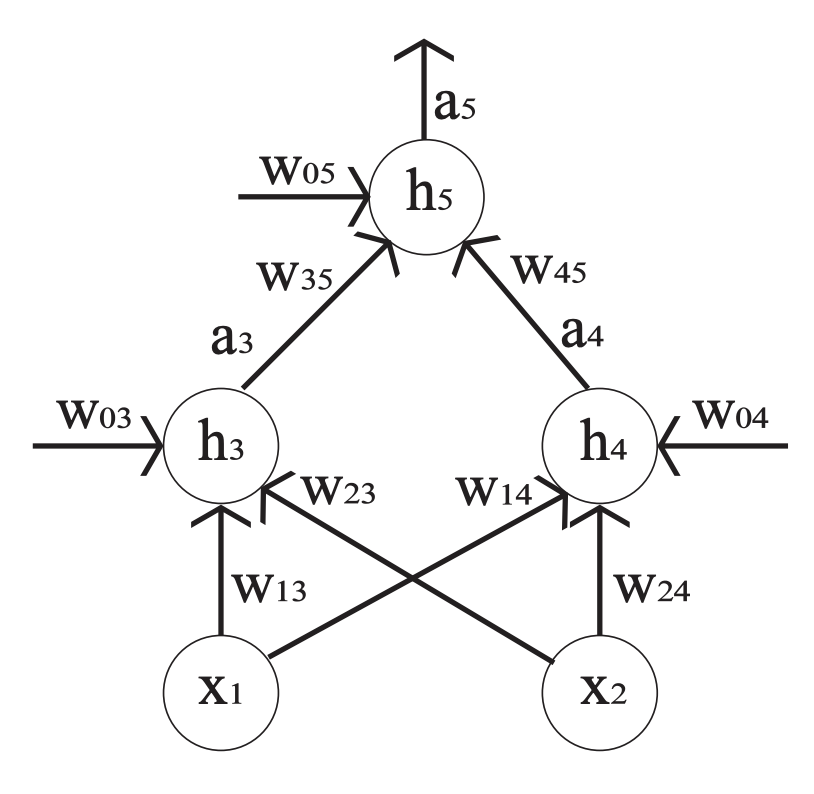
\includegraphics[width=7cm]{figure/p4.png}
    \caption{Multi-layer neural network architecture}
\end{figure}

When an input is passed into a neural network, the signals are passed along the network by following the connections between the units, starting at the input layer and ending in the output layer. This process is referred to as \textbf{forward propagation}. In order for the neural network to learn, it must update its weights across its multiple layers. The common approach for neural network learning is called \textbf{back-propagation}, which relies on the gradient descent method.

\begin{itemize}
\item[(a)]Imagine you are using backprop to do weight updates for an example for which $x_1 = 1$ and $x_2 = -1$. Use $\Delta w_{ij}$ to refer to the amount weight $w_{ij}$ changes as the result of the update. If $\Delta w_{03}$ = $d_3$ and $\Delta w_{04}$ = $d_4$, what are $\Delta w_{13}$, $\Delta w_{23}$, $\Delta w_{14}$, and $\Delta w_{24}$? \defpoints{5}

\item[(b)] This question will have you simulate the process of forward propagation and back-propagation on an example for which $x_1 = 1$ and $x_2 = -1$ and whose desired output is $y = 1$. The values for the various weights are as follows:
\begin{itemize}
\item Weight and bias for $h_3$: $w_{03} = -1$, $w_{13} = 1$, $w_{23} = -1$
\item Weight and bias for $h_4$: $w_{04} = 2, w_{14} = -1, w_{24} = 1$
\item Weight and bias for $h_5$: $w_{05} = -2, w_{35} = 1, w_{45} = 1$
\end{itemize}
For the rest of this question you'll be using the algorithm for forward and back-propagation given in class. Note: \textbf{assume the learning rate $\alpha$ is $0.5$ and Error function for the output is $(\hat{y}-y)^2$.}\\

What is the output and error after the forward propagation? And what is the gradient and updated value after the back-propagation for each weight with the logistic activation function $g(z)=\frac{1}{1+e^{-z}}$? Recall that $g^{\prime}(z)=g(z)(1-g(z))$. Please also give the network's new output and error after the update, and keep your answer to \textbf{three} significant digits after the decimal. \defpoints{15}
\end{itemize}

\solution






\newpage